
\section{Additive Faithfulness}

For general regression, additive approximation may result in a
relevant variable being incorrectly marked as irrelevant. Such
mistakes are inherent to the approximation and may persist even with
infinite samples.  In this section we give
examples of this phenomenon, and then show how the convexity
assumption
changes the behavior of the additive approximation. We begin
with a lemma that characterizes the components of the additive approximation under mild conditions.


% OLD lemma, requires product distribution
% \begin{lemma}
% \label{lem:general_int_reduction}
% Let $F$ be a product distribution on $\mathbf{C}=[0,1]^s$ with density function $p$ which is positive on $\mathbf{C}$. Let
% $X=(X_1,...,X_s) \sim F$. Let $f: \mathbf{C} \rightarrow \R$ be an
% integrable function.
% Let 
% \begin{equation}
% f_k^*, \mu^* \coloneqq \argmin_{f_1,\ldots, f_s, \mu} \Bigl\{ \E \bigl( f(X)  -
%  \sum_{k=1}^s f_k(X_k) -\mu \bigr)^2 
%         \,:\, \E f_k(X_k) = 0\Bigr\}.
% \end{equation}
% Then $\mu^* = \E f(X)$ and $f^*_k(x_k) = \E[ f(X) \given x_k] - \E f(X)$ and this solution is unique.
% \end{lemma}


\begin{lemma}
\label{lem:general_int_reduction}
Let $F$ be a distribution on $C=[0,1]^s$ with a positive density function $p$. Let $f: C \rightarrow \R$ be an integrable function. 

Let $\ds f^*_1,...,f^*_s, \mu^* \coloneqq 
\arg\min \{ \E \big( f(X) - \sum_{k=1}^s f_k(X_k) - \mu \big)^2 \,:\, \forall k, \E f_k(X_k) = 0\}$ 

Then 
$$ f^*_k(x_k) = \E[ f(X) - \sum_{k' \neq k} f^*_{k'}(X_{k'}) \given x_k] - \E f(X) $$
 and $\mu^* = \E f(X)$ and this solution is unique.
\end{lemma}


Lemma~\ref{lem:general_int_reduction} follows from the stationarity
conditions of the optimal solution. 

\begin{proof}
Let $f^*_1,...,f^*_s, \mu^*$ be the minimizers as defined. 

We first show that the optimal $\mu^* = \E f(X)$ for any $f_1, ..., f_k$ such that $\E f_k(X_k) = 0$. This follows from the stationarity condition, which states that $\mu^* = \E[ f(X) - \sum_k f_k(X_k)] = \E[ f(X) ]$. Uniqueness is apparent because the second derivative is strictly larger than 0 and strong convexity is guaranteed.

We now turn our attention toward the $f^*_k$'s. 

It must be that $f^*_k$ minimizes $\Big\{ \E \big( f(X) - \mu^* - \sum_{k' \neq k} f^*_{k'} (X_{k'}) - f_k (X_k) \big)^2 \,:\, \E f_k(X_k) = 0 \Big\}$.

Fix $x_k$, we will show that the value 
$\E[ f(X) - \sum_{k' \neq k} f_{k'}(X_{k'}) \given x_k] - \mu^*$, for all $x_k$,  
uniquely minimizes 
\[
\min_{ f_k(x_k) } \int_{\mathbf{x}_{-k}} p(\mathbf{x}) 
         \Big( f(\mathbf{x}) - \sum_{k' \neq k} f^*_{k'} (x_{k'}) - f_k (x_k) -\mu^*\Big)^2 
                 d \mathbf{x}_{-k}.
\]
It easily follows then that the function $x_k \mapsto \E[ f(X) - \sum_{k'} f_{k'} (X_{k'}) \given x_k] - \mu^*$ is the unique $f^*_k$ that minimizes the expected square error.We focus our attention on $f^*_K$, and fix $x_k$. 

The first-order optimality condition gives us:

\begin{align*}
\int_{\mathbf{x}_{-k}} p(\mathbf{x}) f_k(x_k) d \mathbf{x}_{-k} &= 
  \int_{\mathbf{x}_{-k}} p(\mathbf{x}) 
      ( f(\mathbf{x})-\sum_{k' \neq k} f^*_{k'}(x_{k'})-\mu^*) d \mathbf{x}_{-k} \\  
p(x_k) f_k(x_k) &= \int_{\mathbf{x}_{-k}} p(x_k)
     p(\mathbf{x}_{-k} \given x_k ) 
     ( f(\mathbf{x}) - \sum_{k' \neq k} f^*_{k'} (x_{k'})-\mu^*) 
              d \mathbf{x}_{-k} \\
f_k(x_k) &= \int_{\mathbf{x}_{-k}} 
       p(\mathbf{x}_{-k} \given x_k ) 
     (f(\mathbf{x}) - \sum_{k'\neq k} f_{k'} (x_{k'})  -\mu^*) d \mathbf{x}_{-k} 
 \end{align*}

The square error objective is strongly convex. The second derivative with respect to $f_k(x_k)$ is $2 p(x_k)$, which is always positive under the assumption that $p$ is positive. Therefore, the solution $f^*_k(x_k) = \E[ f(X) \given x_k ] - \E f(X)$ is unique.

Now, we note that as a function of $x_k$, $\E[ f(X) -\sum_{k'\neq k} f_{k'}(X_{k'}) | x_k] - \E f(X)$ has mean zero and we thus finish the proof.
\end{proof}

In the case that the distribution in Lemma~\ref{lem:general_int_reduction} is a product distribution, we get particularly clean expressions for the additive components.

\begin{corollary}
\label{cor:product_int_reduction}
Let $F$ be a product distribution on $\mathbf{C}=[0,1]^s$ with density function $p$ which is positive on $\mathbf{C}$. Let $\mu^*, f^*_k(x_k)$ be defined as in Lemma~\ref{lem:general_int_reduction}.
Then $\mu^* = \E f(X)$ and $f^*_k(x_k) = \E[ f(X) \given x_k] - \E f(X)$ and this solution is unique.
\end{corollary}


If $F$ is the uniform distribution,
then $f^*_k(x_k) = \int f(x_k, \mathbf{x}_{-k})
d\mathbf{x}_{-k}$.

\begin{example} Using Corollary~\ref{cor:product_int_reduction}, we give two examples of \emph{additive unfaithfulness} under
  the uniform distribution, that is, examples where relevant variables are erroneously marked as irrelevant under an additive approximation. First, consider the following function:
\[
\trm{(egg carton)} \quad f(x_1, x_2) = \sin( 2\pi x_1) \sin( 2 \pi x_2)
\]
defined for $(x_1, x_2) \in [0,1]^2$.  Then
$\int_{x_2} f(x_1, x_2) d x_2 = 0$ and
$\int_{x_1} f(x_1, x_2) d x_1 = 0$ for each $x_1$ and $x_2$. An additive approximation
would set $f_1 = 0$ and $f_2 = 0$.  Next, consider the function
\[
\trm{(tilting slope)} \quad f(x_1, x_2) = x_1 x_2
\]
defined for $x_1 \in [-1,1],\; x_2 \in [0,1]$.  In this case
$\int_{x_1} f(x_1, x_2) d x_1 = 0$ for each $x_2$; therefore, we expect $f_2 = 0$ under the additive approximation. This function, for every fixed $x_2$, is a zero-intercept linear function of $x_1$ with slope $x_2$.
\end{example}

\begin{figure*}[htp]
\vskip-10pt
	\centering
	\subfigure[egg carton]{
		\centering
		{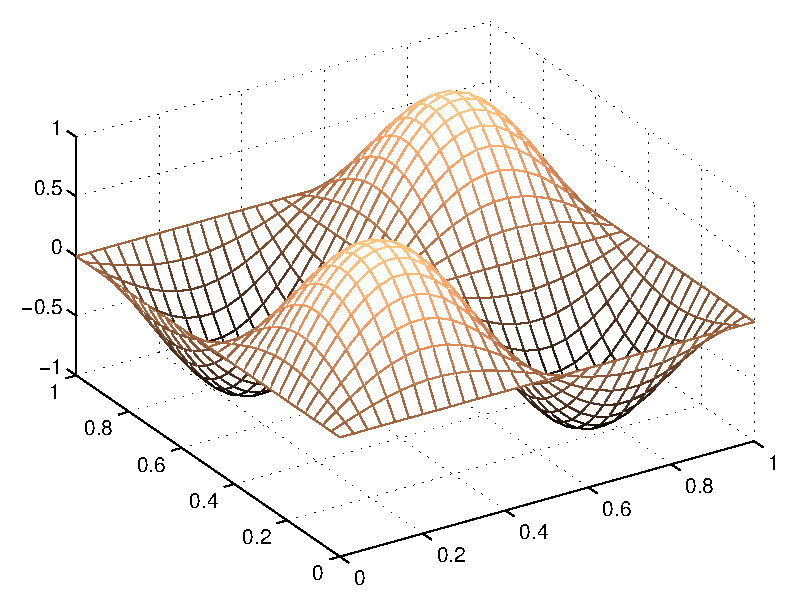
\includegraphics[width=0.4\textwidth]{figs/sine_wave_funct3}}
	}
	\subfigure[tilting slope]{
		\centering
		{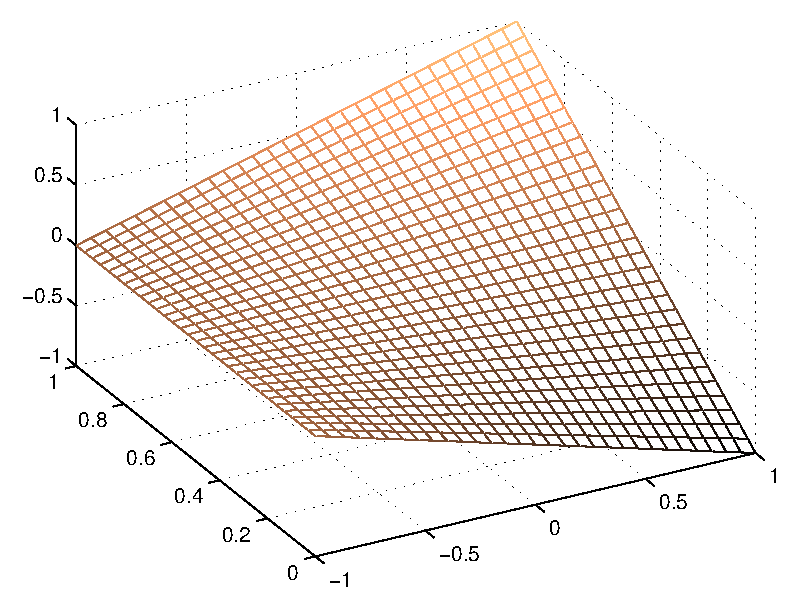
\includegraphics[width=0.4\textwidth]{figs/tilting_slope_funct3}}
	}
\caption{Two additively unfaithful functions. Relevant variables are
  zeroed out under an additive approximation because every ``slice''
  of the function integrates to zero.}
\vskip-10pt
\end{figure*}

In order to exploit additive models, it is important to understand when the
additive approximation accurately captures all of the relevant variables.
We call this property \textbf{additive faithfulness}. We first formalize the intuitive notion that a multivariate function $f$ \emph{depends on} a coordinate $x_k$.

\begin{definition}
  Let $F$ be a distribution on $\mathbf{C}=[0,1]^s$, and $f:\mathbf{C}\rightarrow \R$. 
  
We say that $f$ \textbf{depends on} coordinate $k$ if, for all $x_k \in [0,1]$, the set 
$\big\{ x'_k \in [0, 1] \,:\, f(x_k, \mathbf{x}_{-k}) = f(x'_k, \mathbf{x}_{-k}) 
\trm{ for almost all  $\mathbf{x}_{-k}$} \big\}$ 
has measure strictly less than 1.\\

Suppose we have the additive approximation:
\begin{equation}
f_k^*, \mu^* \coloneqq \argmin_{f_1,\ldots, f_s, \mu} \Bigl\{ 
             \E ( f(X) - \sum_{k=1}^s f_k(X_k) -\mu )^2 
         \,:\, \E f_k(X_k) = 0 \Bigr\}.
\end{equation}
We say that $f$ has \textbf{additive recall} under $F$ if $f^*_k = 0 \Rightarrow \trm{$f$ does not depend on coordinate $k$}$. 

We say that $f$ is \textbf{additively faithful} under $F$ in case $f^*_k = 0$ iff $f$ does not depend on coordinate $k$. 
\end{definition}
% We can define the support $\trm{supp}(f) \coloneqq \{ k \,:\,
% \trm{$k$ is relevant to $f$}\}$. Let $f^* = \sum_{k=1}^s$, then $f$
% is additively faith if $\trm{supp}(f) = \trm{supp}(f^*)$.

Additive faithfulness is an attractive property because it implies that, in the population setting, the additive approximation yields consistent variable selection. Additive recall is a weaker condition but still useful: we can be sure that the additive approximation is conservative, that it does not exclude important variables.

Remarkably, under a general class of distributions which we characterize below, convex multivariate functions has additive recall and under product distributions, convex functions are additively faithful.

\begin{definition}
Given a conditional density $p(\mathbf{x}_{-j} \given x_j)$, we say that $\mathbf{X}_{-j}$ is \textbf{intermittently independent} of $X_j$ if the set of $x_j$ for which $\frac{\partial p(\mathbf{x}_{-j} \given x_j)}{\partial x_j} = 0$ for all $\mathbf{x}_{-j}$ is either the whole line $[0,1]$, or a collection of at least two disjoint closed intervals.

Let $F$ be a distribution on $[0,1]^s$. We say that $F$ is an \textbf{intermittently independent} distribution if $F$ has a non-zero density $p$ with the property that, for all $j=1,...,s$, $\mathbf{X}_{-j}$ is intermittently independent of $X_j$.
\end{definition}

\begin{example} There are many examples of distributions which satisfy intermittent independence:
\begin{packed_enum}
\item $F$ is a product distribution.
\item $F$ has a density $p$ that is piece-wise constant on a gridding of $[0,1]^s$.
\item $F$ has a density $p$ that is, for some $\frac{1}{2} > \epsilon > 0$,  arbitrary on $(\epsilon, 1-\epsilon)^s$ but constant elsewhere. 
\end{packed_enum}
\end{example}

\begin{theorem}
\label{thm:convex_recall}
Let $F$ be an \textbf{intermittently independent} distribution supported on $C=[0,1]^s$ with positive density $p$. If $f$ is convex and twice differentiable, then $f$ has the \emph{additive recall} property under $F$.
\end{theorem}

\begin{theorem}
\label{thm:convex_faithful}
Let $F$ be a product distribution supported on $C=[0,1]^s$ with positive density $p$. If $f$ is convex and twice differentiable, then $f$ is \emph{additively faithful} under $F$.
\end{theorem}


% We give the full proof in Section~\ref{sec:faithful_proof} of the
% Appendix, but pause here to provide some intuition. 

In the case of Theorem~\ref{thm:convex_faithful}, we can give some intuition: Lemma~\ref{lem:general_int_reduction}, we know that the
additive approximation zeroes out $k$ when, fixing $x_k$, every
``slice'' of $f$ integrates to zero. We prove
Theorem~\ref{thm:convex_faithful} by showing that ``slices'' of convex
functions that integrate to zero cannot be ``glued'' together while
still maintaining convexity.

We give the proof of Theorem~\ref{thm:convex_recall}, which also proves one direction of Theorem~\ref{thm:convex_faithful}. The other direction of Theorem~\ref{thm:convex_faithful} is trivial to show.

\begin{proof} (of Theorem~\ref{thm:convex_recall})\\
Fix $k$. Using the result of Lemma~\ref{lem:general_int_reduction}, we need only show that for all $x_k$, $ \E[ f(X) - \sum_{k'} f_{k'}(X_{k'}) \given x_k] - \E f(X) = 0 $ implies that $f$ does not depend on coordinate $k$.\\

By assumption, we know that there exist at least two disjoint closed intervals $R_0, R_1$ where $p(\mathbf{x}_{-k} \given x_k)$ is independent on $x_k$. That is, there exist density functions $\phi_0(\mathbf{x}_{-k})$ and $\phi_1(\mathbf{x}_{-k})$ such that $p(\mathbf{x}_{-k} \given x_k) = \phi_0(\mathbf{x}_{-k})$ for all $x_k \in R_0$ and $p(\mathbf{x}_{-k} \given x_k) = \phi_1(\mathbf{x}_{-k})$ for all $x_k \in R_1$.


Let $x^0_k$ be an interior point of $R_0$. 

For every $\mathbf{x}_{-k}$, we define $g$ as the derivative of $f$ with respect to $x_k$ at the point $(\mathbf{x}_{-k}, x^0_k)$.
\[
g(\mathbf{x}_{-k}) \coloneqq  \lim_{x_k \rightarrow x^0_k} 
     \frac{f(x_k, \mathbf{x}_{-k}) - f(x^0_k, \mathbf{x}_{-k})}{x_k - x^0_k}
\]
$g(\mathbf{x}_{-k})$ is well-defined by the assumption that $f$ is everywhere differentiable.

Now, we use $r(\mathbf{x}_{-k})$ as a short-hand for $\sum_{k'\neq k} f_{k'}(x_{k'})$ and derive that for all $x_k \in R_0$, we have:
\begin{align*} 
& \int_{\mathbf{x}_{-k}}  \phi_0(\mathbf{x}_{-k}) 
   \Big( f(x_k, \mathbf{x}_{-k}) - f(x_k^0, \mathbf{x}_{-k}) \Big) d\mathbf{x}_{-k} \\
 &= \int_{\mathbf{x}_{-k}}  \phi_0(\mathbf{x}_{-k})
   \Big( \big(f(x_k, \mathbf{x}_{-k}) - r(\mathbf{x}_{-k}) - \mu^* \big) - 
         \big(f(x^0_k, \mathbf{x}_{-k}) - r(\mathbf{x}_{-k}) - \mu^* \big) \Big)
     d \mathbf{x}_{-k} \\
 &= 0
\end{align*}

Since $x^0_k$ is in the interior of $R_0$, we use the bounded convergence theorem and conclude that $\int_{\mathbf{x}_{-k}} \phi_0( \mathbf{x}_{-k}) g(\mathbf{x}_{-k}) = 0$ as well.

We now note that $g(\mathbf{x}_{-k})$ is a component of the subgradient 
$\partial_{\mathbf{x}} f(x^0_k, \mathbf{x}_{-k})$. 

Therefore, the first-order characterization of convex functions gives us that
\begin{align*}
f(x_k, \mathbf{x}_{-k}) \geq f(x^0_k, \mathbf{x}_{-k}) + g(\mathbf{x}_{-k}) (x_k - x^0_k)
   \quad \trm{for all } x_k, \mathbf{x}_{-k}
\end{align*}

Or, equivalently, for all $x_k, \mathbf{x}_{-k}$, 
\[
f(x_k, \mathbf{x}_{-k}) - f(x^0_k, \mathbf{x}_{-k}) - g(\mathbf{x}_{-k}) (x_k-x^0_k) \geq 0
\]

Now, for all $x_k \in R_0$, 
\[
\int_{\mathbf{x}_{-k}} \phi_0(\mathbf{x}_{-k}) 
     \Big(f(x_k, \mathbf{x}_{-k}) - f(x^0_k, \mathbf{x}_{-k}) 
     - g(\mathbf{x}_{-k}) (x_k - x^0_k) \Big) d\mathbf{x}_{-k} = 0
\]
Since $\phi_0$ is positive by assumption, we conclude that for all $x_k \in R_0$, for all $\mathbf{x}_{-k}$, 
$$
f(x_k, \mathbf{x}_{-k}) = f(x^0_k, \mathbf{x}_{-k}) - g(\mathbf{x}_{-k}) (x_k - x^0_k)
$$

The Hessian of $f$ at $(x_k, \mathbf{x}_{-k})$ for $x_k \in R$ then has a zero at the $k$-th main diagonal entry. A positive semidefinite matrix with a zero on the $k$-th main diagonal entry must have only zeros on the $k$-th row and column \footnote{ See proposition 7.1.10 of \citet{HJ90}}, which means that $g(\mathbf{x}_{-k})$ must be a constant function. Since $g$ integrates to 0 under $\phi_0(\mathbf{x}_{-k})$, it must be 0.\\

Thus, $f(x_k, \mathbf{x}_{-k}) = f(x^0_k, \mathbf{x}_{-k})$ for all $x_k \in R_0$ and for all $\mathbf{x}_{-k}$.\\

We can go through the same reasoning for $R_1$  and get that $f(x_k, \mathbf{x}_{-k})$ is a constant function of $x_k$ for all $x_k \in R_1$, that is, $f(x_k, \mathbf{x}_{-k}) = f(x^1_k, \mathbf{x}_{-k})$ for all $x_k \in R_1$ for some interior point $x^1_k$ of $R_1$.

However, if $f(x_k, \mathbf{x}_{-k})$, as an one-dimensional convex function of $x_k$, is constant on two disjoint closed intervals, it must be constant for all $x_k \in [0,1]$. Therefore, for all $\mathbf{x}_{-k}$, $f(x_k, \mathbf{x}_{-k})$ is a constant as a function of $x_k$ and $f$ does not depend on $x_k$.

\end{proof}

Theorem~\ref{thm:convex_faithful} plays an important role in our
sparsistency analysis, where we show that the additive
approximation is variable selection consistent (or ``sparsistent''), even when the true function is not
additive.

\begin{remark}
  We assume twice differentiability in
  Theorems~\ref{thm:convex_faithful} and~\ref{thm:convex_recall} to simplify the proof. 
  We believe
  this smoothness condition is not necessary because every non-smooth
  convex function can be approximated arbitrarily well by a smooth
  one.  
\end{remark}

% \begin{remark}
% Without restrictions on the distribution, a convex
%   function may not be additively faithful. Intuitively, an arbitrarily shaped
%   density $p$
%   may ``undo'' the convexity of $f$ so that the product
%   $p(\mathbf{x}) \, f(\mathbf{x})$ resembles an egg carton or a
%   tilting slope.  With appropriate conditions on the density $p$,
%   however, it is possible to relax the independence assumption.  We leave this to
%   future work.
% \end{remark}


% DO NOT CHANGE; RefTex variables -minx
 
%%% Local Variables: ***
%%% mode:latex ***
%%% TeX-master: "paper.tex" ***
%%% End: ***

